\documentclass[border=2]{standalone}
\usepackage[utf8]{inputenc}

\usepackage{tikz, times}
\usetikzlibrary{mindmap, backgrounds}

\begin{document}
\centering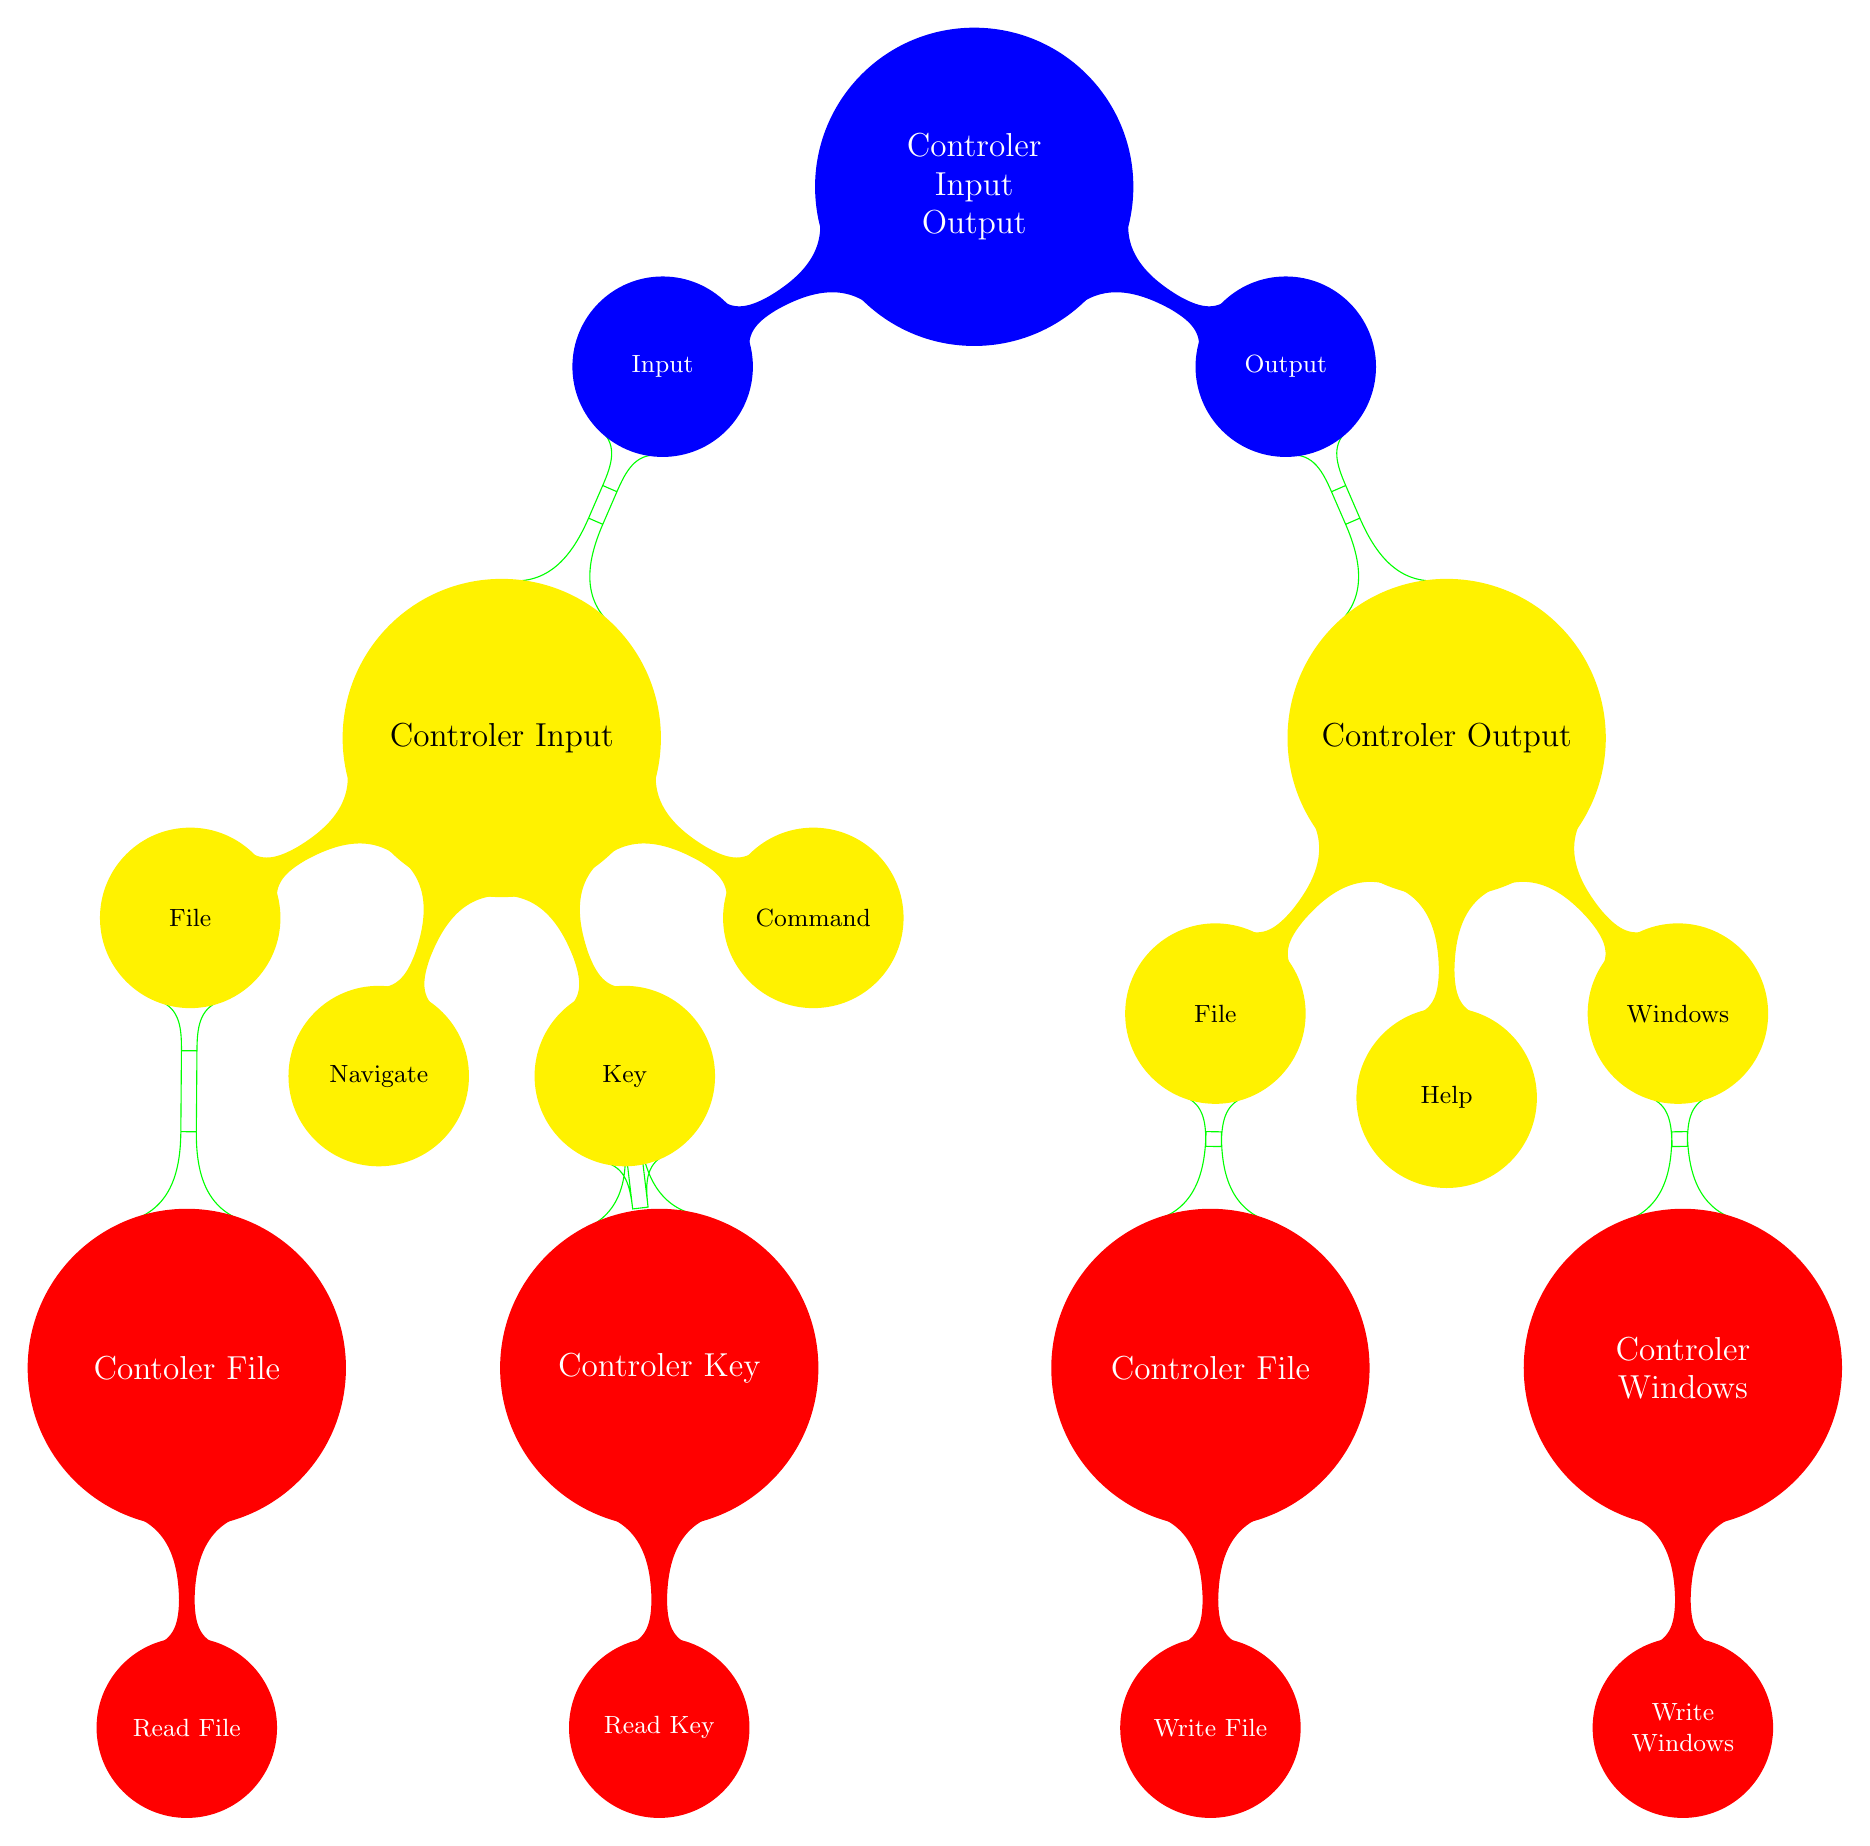
\begin{tikzpicture}[mindmap,% No pillo que fa xD
	level 1 concept/.append style={level distance=130,sibling angle=30},
	extra concept/.append style={color=blue!50,text=black}]

% El primer de tots, el controlador dels grans controladors
\begin{scope}[mindmap, concept color=blue, text=white]
\node [concept] {Controler\\Input\\Output} [clockwise from=-5]% ni idea
	child [grow=-150]	{node [concept] (Input)		{Input}}
	child [grow=-30]	{node [concept]	(Output)	{Output}};
\end{scope}
%%%%%%%%%%%%%%%%%%%%%%%%%%%%%%%%%%%%%%%%%%%%%%%%%%%%%%%%%%%%%%%%%%%%%%%%%%%%%%%%%%%%%%%%%%%%%%%%%%%%%%%%%%%%%%%%%%%%%%%%%%%%%%%%
\begin{scope}[mindmap, concept color=yellow]
\node [concept] (CI) at (-6, -7) {Controler Input}
	child [grow=-150]	{node [concept] (IFile)		{File}}
	child [grow=-110]	{node [concept]			{Navigate}}
	child [grow=-70]	{node [concept] (Key)		{Key}}
	child [grow=-30]	{node [concept]			{Command}};
\end{scope}
\begin{scope}[mindmap, concept color=red, text=white]
\node [concept] (ICF) at (-10, -15) {Contoler File}
	child	{node [concept]	{Read File}};
\end{scope}
\begin{scope}[mindmap, concept color=red, text=white]
\node [concept] (ICK) at (-4, -15) {Controler Key}
	child	{node [concept]	{Read Key}};
\end{scope}
%%%%%%%%%%%%%%%%%%%%%%%%%%%%%%%%%%%%%%%%%%%%%%%%%%%%%%%%%%%%%%%%%%%%%%%%%%%%%%%%%%%%%%%%%%%%%%%%%%%%%%%%%%%%%%%%%%%%%%%%%%%%%%%%
\begin{scope}[mindmap, concept color=yellow]
\node [concept] (CO) at (6, -7) {Controler Output}
	child [grow=-90]	{node [concept] {Help}}
	child [grow=-130]	{node [concept] (OFile)		{File}}
	child [grow=-50]	{node [concept] (Windows)	{Windows}};
\end{scope}
\begin{scope}[mindmap, concept color=red, text=white]
\node [concept] (OCF) at (3, -15) {Controler File}
	child	{node [concept] {Write File}};
\end{scope}
\begin{scope}[mindmap, concept color=red, text=white]
\node [concept] (CW) at (9, -15) {Controler Windows}
	child {node [concept] {Write Windows}};
\end{scope}
%%%%%%%%%%%%%%%%%%%%%%%%%%%%%%%%%%%%%%%%%%%%%%%%%%%%%%%%%%%%%%%%%%%%%%%%%%%%%%%%%%%%%%%%%%%%%%%%%%%%%%%%%%%%%%%%%%%%%%%%%%%%%%%%

%%%%%%%%%%%%%%%%%%%%%%%%%%%%%%%%%%%%%%%%%%%%%%%%%%%%%%%%%%%%%%%%%%%%%%%%%%%%%%%%%%%%%%%%%%%%%%%%%%%%%%%%%%%%%%%%%%%%%%%%%%%%%%%%
% Connecions
%%%%%%%%%%%%%%%%%%%%%%%%%%%%%%%%%%%%%%%%%%%%%%%%%%%%%%%%%%%%%%%%%%%%%%%%%%%%%%%%%%%%%%%%%%%%%%%%%%%%%%%%%%%%%%%%%%%%%%%%%%%%%%%%
\begin{pgfonlayer}{background}
\draw [circle connection bar, fill=red, draw=green]
	(Input)		edge (CI)
	(Key)		edge (ICK)
	(IFile)		edge (ICF)

	(Output)	edge (CO)
	(OFile)		edge (OCF)
	(Windows)	edge (CW);
\end{pgfonlayer}

\end{tikzpicture}
\end{document}
